% !TEX encoding = UTF-8 Unicode
% !TEX root = SystemTemplate.tex

\documentclass{book}
% !TEX root = SystemTemplate.tex

\usepackage[width=6.5in, height=9.2in, top=1.0in, papersize={8.5in,11in}]{geometry}
\usepackage[pdftex]{graphicx}
%\usepackage{draftwatermark}
\usepackage{amsmath}
\usepackage{amsthm}
\usepackage{amssymb}
%\usepackage{txfonts}
\usepackage{textcomp}
%\usepackage{amsthm}

\usepackage[all]{xy}
\usepackage{fancyhdr}
\pagestyle{fancy}
\usepackage{hyperref}
\usepackage{verbatim}
\usepackage{algorithm}
\usepackage{algorithmic}
\usepackage{array}
\usepackage{color}
\usepackage{listings}
\lstset{language=c,frame=ltrb,framesep=5pt,basicstyle=\normalsize,
 keywordstyle=\ttfamily\color{DarkRed},
identifierstyle=\ttfamily\color{DarkBlue}\bfseries,
commentstyle=\color{OliveGreen},
stringstyle=\ttfamily,
showstringspaces=false,tabsize = 3}
\usepackage{calc}
\usepackage{doxygen}
\usepackage[utf8]{inputenc}
\usepackage{makeidx}
\usepackage{multicol}
\usepackage{multirow}
\usepackage[table]{xcolor}

\definecolor{color02}{rgb}{0.18,0.35,0.59}
\definecolor{color03}{rgb}{0.44,0.59,0.82}
\definecolor{color06}{rgb}{0.35,0.35,0.35}


\newtheorem{summary}{Summary:}
\newtheorem{example}{Example:}


\definecolor{OliveGreen}{cmyk}{0.64,0,0.95,0.40}
\definecolor{DarkBlue}{cmyk}{0.76,0.76,0,0.20}
\definecolor{DarkRed}{cmyk}{0,1,1,0.45}


\def      \RR             {{\mathbb R}} 
\def      \DS            {\displaystyle} 

\setlength{\oddsidemargin}{0mm} 
\setlength{\evensidemargin}{0mm} 

%\SetWatermarkLightness{0.975}
%\SetWatermarkScale{6}
%\SetWatermarkText{\includegraphics{test.png}}

\pagestyle{fancy}
\renewcommand{\chaptermark}[1]{\markboth{#1}{}}
\renewcommand{\sectionmark}[1]{\markright{\thesection\ #1}}
\fancyhf{}
\fancyhead[LE,RO]{\bfseries\thepage}
\fancyhead[LO]{\bfseries\rightmark}
\fancyhead[RE]{\bfseries\leftmark}
\fancyfoot[LE,RO]{Confidential and Proprietary}
%\renewcommand{\headrulewidth}{0.5pt}
%\renewcommand{\footrulewidth}{0pt}
%\addtolength{\headheight}{0.5pt}
%\setlength{\footskip}{0mm}
%\renewcommand{\footruleskip}{0pt}


\definecolor{MSBlue}{rgb}{.204,.353,.541}
\definecolor{MSLightBlue}{rgb}{.31,.506,.741}
\definecolor{MSBlue1}{rgb}{0.18,0.35,0.59}
\definecolor{MSBlue2}{rgb}{0.44,0.59,0.82}
\definecolor{MSBlue3}{rgb}{0.35,0.35,0.35}


\usepackage{titlesec}
\titleformat{\chapter}[display]
{\normalfont\bfseries\color{MSBlue1}}    %\normalfont\bfseries\filcenter}
{\LARGE\thechapter}
{1ex}
{\titlerule[2pt]
\vspace{2ex}%
\LARGE}
[\vspace{1ex}%
{\titlerule[2pt]}]

\definecolor{MSBlue}{rgb}{.204,.353,.541}
\definecolor{MSLightBlue}{rgb}{.31,.506,.741}
\definecolor{MSBlue1}{rgb}{0.18,0.35,0.59}
\definecolor{MSBlue2}{rgb}{0.44,0.59,0.82}
\definecolor{MSBlue3}{rgb}{0.35,0.35,0.35}

%\titleformat*{\section}{\Large\bfseries\sffamily\color{MSBlue}}
%\titleformat*{\subsection}{\large\bfseries\sffamily\color{MSLightBlue}}
%\titleformat*{\section}{\Large\bfseries\color{MSBlue1}}
%\titleformat*{\subsection}{\large\bfseries\color{MSBlue2}}

\titleformat*{\section}{\Large\bfseries\color{MSBlue}}
\titleformat*{\subsection}{\large\bfseries\color{MSLightBlue}}
\titleformat*{\subsubsection}{\large\bfseries\color{MSBlue3}}
\setcounter{secnumdepth}{3}
\renewcommand{\thesubsubsection}{\thesubsection.\alph{subsubsection}}

 % This sets the format.

% Add your title page contents here 
\title{{\color{MSBlue1} \rule{\linewidth}{0.5mm}}\\[2mm] {\huge \bfseries \color{MSBlue1} Autotester }\\[-1mm] {\color{MSBlue1}\rule{\linewidth}{0.5mm}} \\  \vfill
{\LARGE \bfseries \color{MSBlue2} Senior Design Final Documentation }\\  \vfill 
{\color{MSBlue1} Whitespace Cowboys} }
\author{\color{MSBlue1}  Ryan Feather \and \color{MSBlue1} Ryan Brown \and  \color{MSBlue1} Kelsey Bellew \and  \color{MSBlue1} (Inherited from)The Obfuscators }
\date{\color{MSBlue1} \today}


\begin{document}
\frontmatter
\maketitle


\tableofcontents
\listoffigures
\listoftables
\listofalgorithms


% !TEX root = SystemTemplate.tex

\chapter{Mission}

To design and implement an automatic testing system that will completely and effectively meet all of the needs of our client  % add mission statement to mission.tex
% !TEX root = SystemTemplate.tex

\chapter{Document Preparation and Updates}

Current Version [1.0.4]
\vspace*{5mm}

{\color{MSBlue3}
\noindent
\textit{Prepared By:}\\
\textit{Daniel Nix}\\
\textit{Joseph Lillo}\\
\textit{Elizabeth Woody}
}

\vfill
\noindent
{\color{color02} \textit{\textbf{Revision History}}}\\
\begin{tabular}{|>{\raggedright}p{1.5cm}|>{\raggedright}p{3cm}|>{\raggedright}p{1.5cm}|>{\raggedright}p{9cm}|}
\hline
\textit{\textbf{Date}} &  \textit{\textbf{Author}} & \textit{\textbf{Version}} & \textit{\textbf{Comments}}\tabularnewline
\hline
 \textit{\textbf{2/6/14}} & \textit{Elizabeth Woody} & \textit{1.0.0} & \textit{Initial version}\tabularnewline
\hline
\textit{\textbf{2/13/14}} & \textit{Obfuscators} & \textit{1.0.1} & \textit{Edited version}\tabularnewline
\hline
 \textit{\textbf{2/16/14}} & \textit{Lillo, Woody} & \textit{1.0.2} & \textit{Edited version}\tabularnewline
 \hline
 \textit{\textbf{2/17/14}} & \textit{Daniel Nix} & \textit{1.0.3} & \textit{Edited version}\tabularnewline
\hline
 \textit{\textbf{2/18/14}} & \textit{Obfuscators} & \textit{1.0.4} & \textit{Final version}\tabularnewline
\hline
 &  &  & \tabularnewline
\hline
 &  &  & \tabularnewline
\hline
\end{tabular}
\vfill



 
\mainmatter

%%  Add to the following chapters

% !TEX root = SystemTemplate.tex

\chapter{Overview and concept of operations}


\section{Scope}
This document will provide an overview of the develolpment of the testing software.


\section{Purpose}
This product will compile and test c++ programs against predefined test cases.


\subsection{Major System Component \#1}
Location of existing, applicable test cases for the program needing to be tested.

\subsection{Major System Component \#2}
Run and test of a single program against located test cases

\subsection{Major System Component \#3}
Record and summary of test results

\section{Systems Goals}
The goal of this system is to provide an automated testing application, designed specifically
for professors testing submitted student programs. A user will be able to use the application
to test a desired program against all applicable test cases the application can find in the directory tree 
related to that program.  A time-stamped record will be created to summarize the output of each test and to provide a
general summary of the results. 

\section{System Overview and Diagram}
The major system components listed above will, upon completion, combine to create this testing application. 
Upon running the application and providing it with the name of the desired target program, the application
will complete the desired system goals via its major components.
\\ First, existing, applicable test cases will be found for the program needing to be tested. 
\\ Second, the program will be run against each test case input, and the resulting output will be 
compared to each desired test case output.
\\  Last, the program will create a time-stamped record for each program tested, providing a reference of 
the output results and a numerical summary of the overall success rate.  
\\ See Figure~\ref{systemdiagram}.
\begin{figure}[H]
\begin{center}
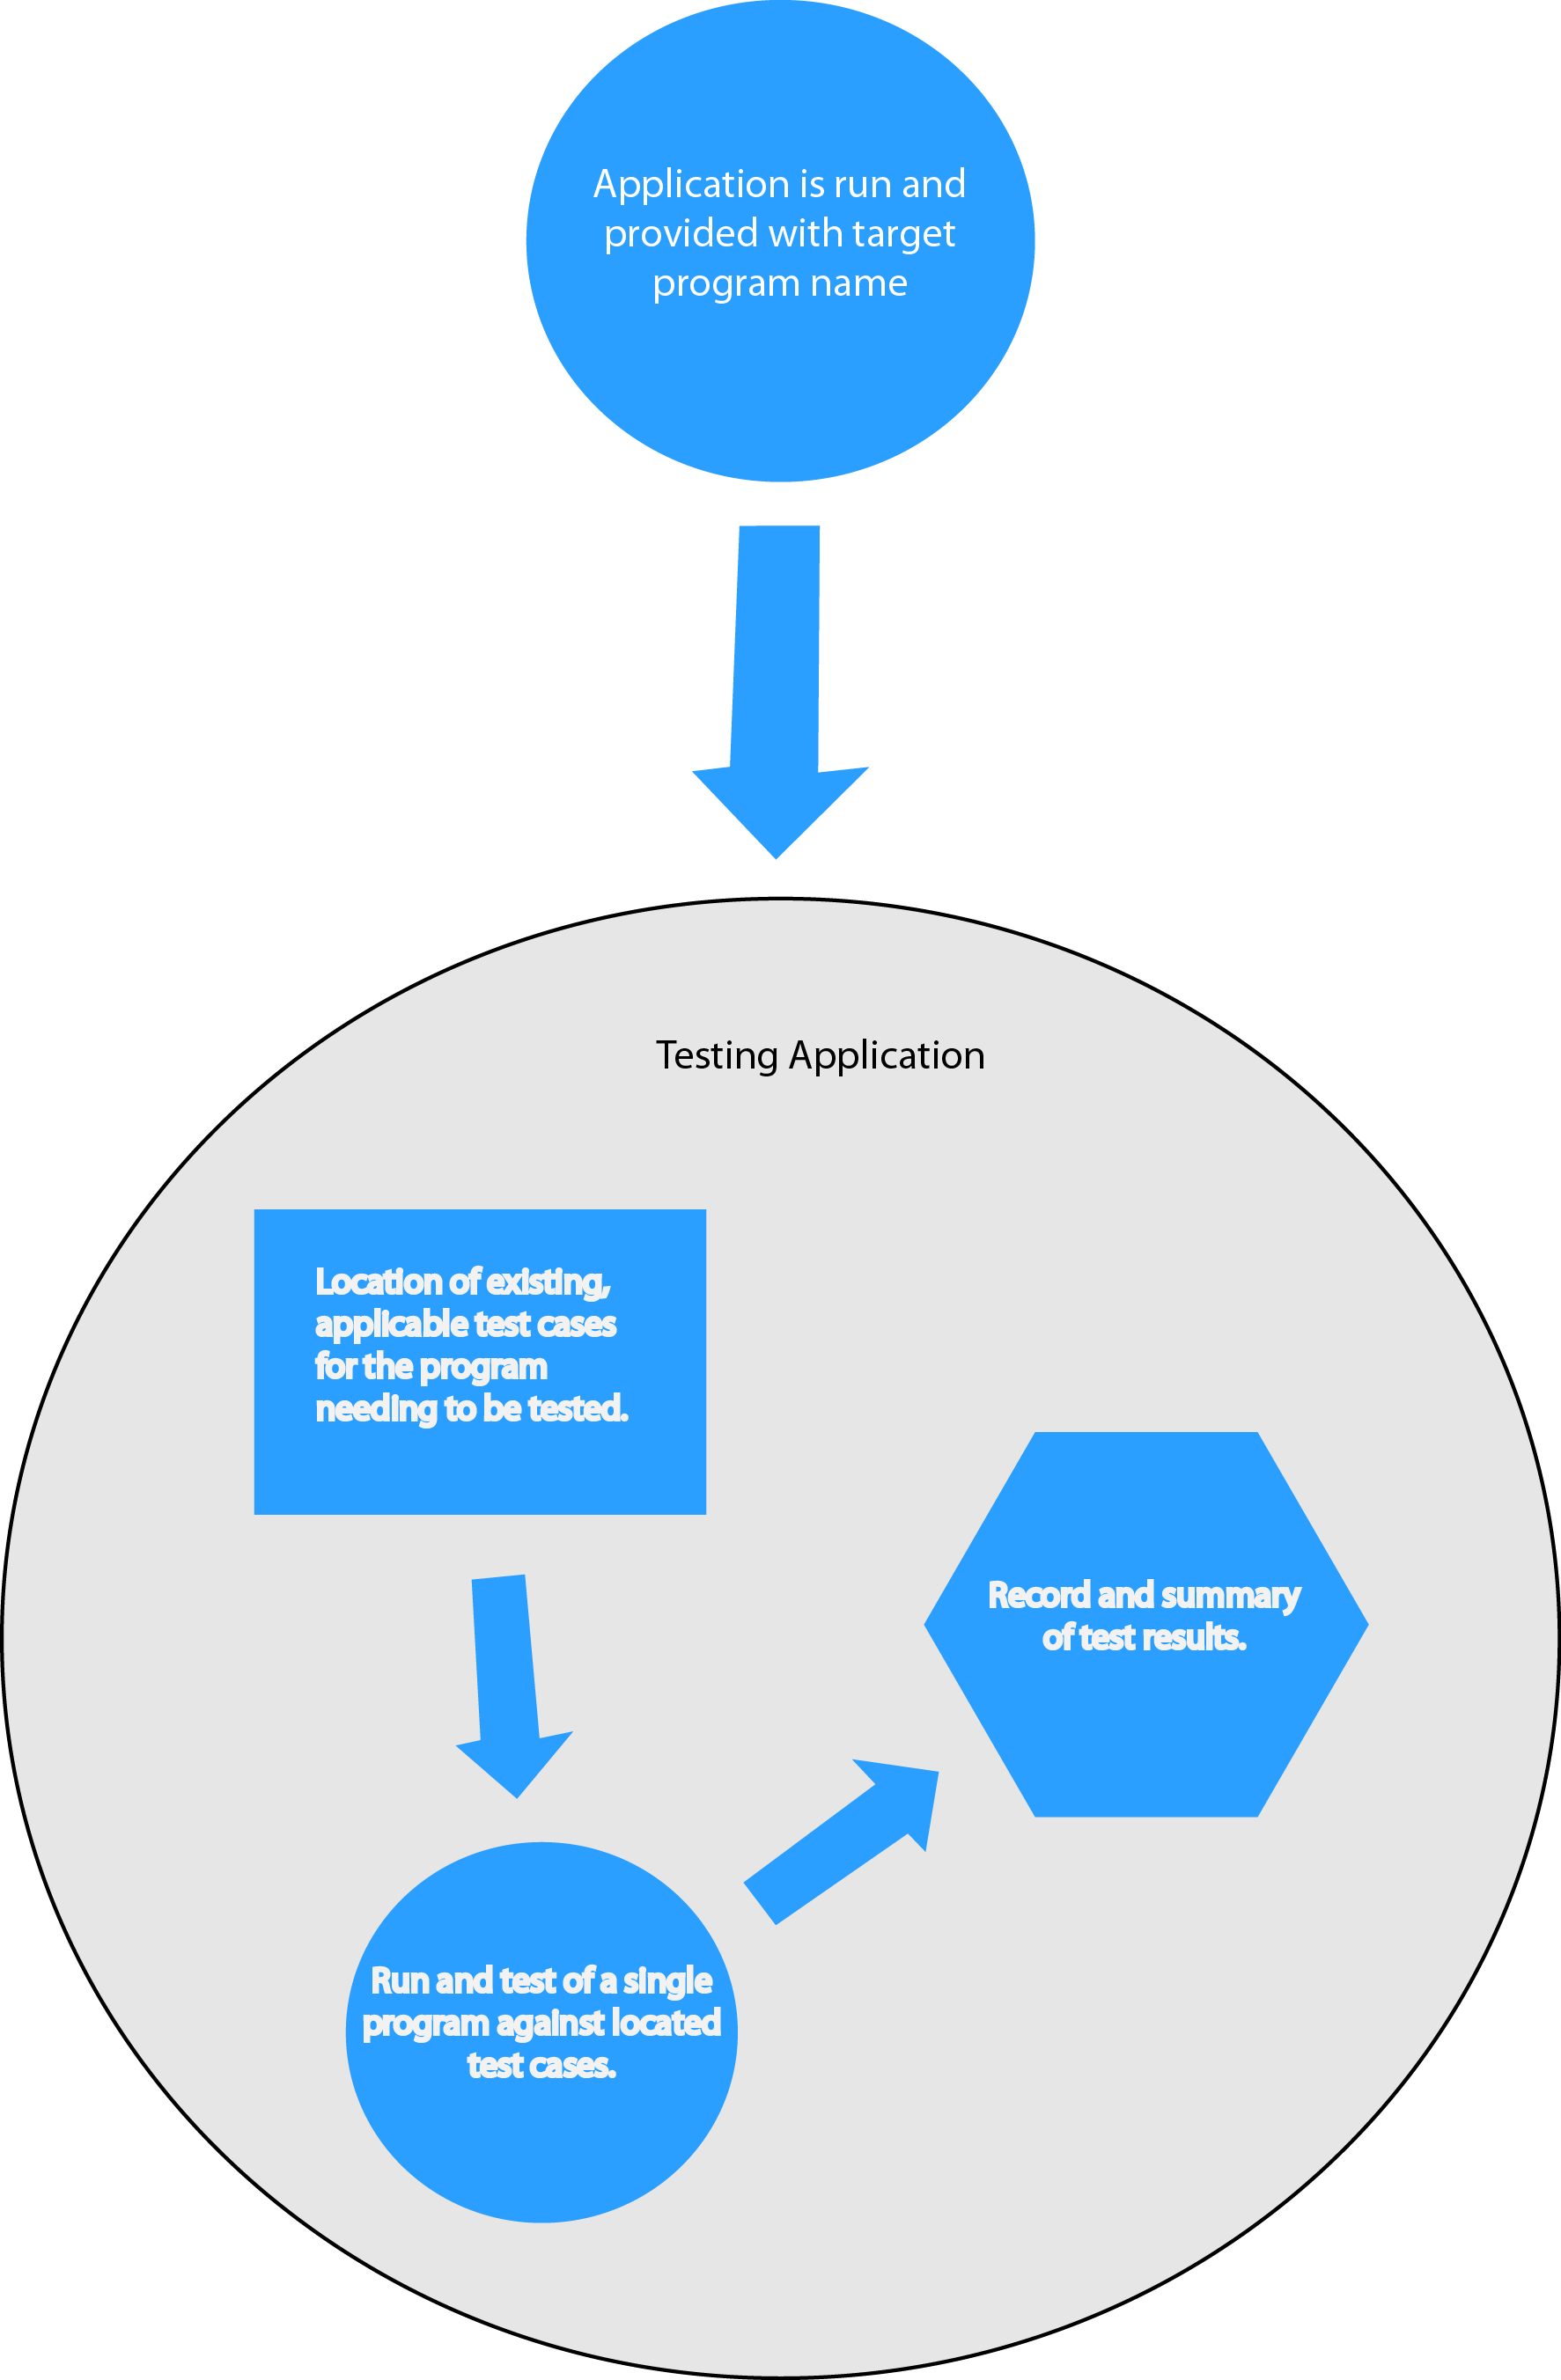
\includegraphics[width=0.9\textwidth]{./diagram}
\end{center}
\caption{The Testing System Diagram \label{systemdiagram}}
\end{figure}



\section{Technologies Overview}
The development team used the Agile Software Development Method, via the Scrum framework, to develop
this system.  This incremental development menthod was the required development method for this project.
Since the system was expected to created for a Linux platform, it was written and tested on a Linux Platform 
using Qt Creator.  The latter was picked as the Integrated Development Environment of the system, based on
the requirement that it be written in the programing language C++.
See Table~\ref{DevelopmentTable}.  
\begin{table}[tbh]
\begin{center}
\begin{tabular}{|r|l|}
  \hline
  Software Development Method & Agile Software Development Method \\
  Planning and Organization & Trello Project Management Application \\
  \hline \hline
  Platform & Linux \\
  Language & C++ \\  
  IDE & Qt Creator \\
  Version Control & Git and Bitbucket
  \\ \cline{2-2}
  
  \hline
\end{tabular}
\caption{The Development Methods and Technologies Table \label{DevelopmentTable}}
\end{center}
\end{table}


% !TEX root = SystemTemplate.tex


\chapter{Project Overview}
This section provides some housekeeping type of information with regard to the 
team, project, etc. 



\section{Team Members and Roles}
\subsection{Obfuscators}
\begin{description}
\item[$\bullet$ ] Joseph Lillo - Technical Lead
\item[$\bullet$ ] Daniel Nix - Product Owner
\item[$\bullet$ ] Lisa Woody - Scrum Master
\end{description}
\subsection{Whitespace Cowboys}
The team members of the Whitespace Cowboys were Kelsey Bellew, Ryan Brown, and Ryan Feather. 

\begin{itemize}
\item Kelsey Bellew was the Scrum Master.
\item Ryan Brown was the Product Owner.
\item Ryan Feather was the Technical Lead.
\end{itemize}

\subsection{Kernel\_Panic}
The team members of Kernel\_Panic were Anthony Morast, Benjamin Sherman, and James Tillma.

\begin{itemize}
\item Anthony Morast - Technical Lead
\item Benjamin Sherman - Product Owner
\item James Tillma - Scrum Master
\end{itemize}


\section{Project  Management Approach}
This project was managed using the Agile Software Development Method, via the Scrum framework.
Trello, a web-based project management application, was used to assign tasks and keep track of 
the product backlog.  For version control, Git was used.

The sprint length for the development of this system was three weeks, with
only one sprint being necessary for completion.  The user stories were provided by the product 
owner, Benjamin Sherman, who actively communicated with the future application user.  These were used
to create the product backlog and to determine the requirements and components of the system.


\section{Phase  Overview}
The program was developed through four different phases:
\begin{description}
\item[1. ] Implement a directory crawl to find all of the test cases.
\item[2. ] Run the program to be tested, using the input from the test case. Store the result in an output file.
\item[3. ] For each test case found, compare the tested program's output file to the desired output file (included with each test case).
\item[4. ] Create a time-stamped log file to retain the output files and results of the test.  This will include a record of the success and failure rate of the test.
\item[5. ] Generate test files and create answer files. Answer files will be generated when the test files are piped into the golden cpp file.
\item[6. ] Add profiling and code coverage functionality.
\item[7. ] Modify \textit{diff} to the effect that student solutions need not be exact matches to the answer.
\item[8. ] Limit runtime of a student program. Consider the student program to be in an infinite loop if it runs too long.
\end{description}


\section{Terminology and Acronyms}
See Table \ref{terms}
\begin{table}[tbh]
\begin{center}
\begin{tabular}{|r|l|}
\hline
    GNU and GNU Tools & The tools provided in most GNU\textbackslash Linux environments \\ \hline
    Agile Methodology & An approach to project management and software development \url{agilemanifesto.org} \\ \hline
    C++ Template Libraries & A built-in set of classes used for storing data. \\ \hline
    GCOV & GNU C++ code coverage utility \\ \hline
    GPROF & GNU C++ code profiling utility \\
    \hline
\end{tabular}
\caption{Defining Some Important Terms \label{terms}}
\end{center}
\end{table}

% !TEX root = SystemTemplate.tex
\chapter{User Stories, Backlog and Requirements}
\section{Overview}
This section contains several user stories, a backlog, and a list of requirements, of
both the project and the user, and the user's equiptment for using the project. This
chapter will contain 
details about each of the requirements and how the requirements are or will be 
satisfied in the design and implementation of the system.

The user stories are provided by the stakeholders.

\subsection{Scope}

This document will contain stakeholder information, initial user stories, requirements, and 
proof of concept results.



\subsection{Purpose of the System}
The purpose of the product is to allow the user to run pre-written and product generated auto tests on a directory or 
program of their choosing, and to provide a log to the user of which tests passed and which tests failed for each program 
that is found within the given directory. A PASS, FAIL, and or percentage is written to a log placed within a found 
program's directory. 

In addition, the purpose of the product is to allow the user to generate a given number of random 
tests with user given parameters.

\section{ Stakeholder Information}


\subsection{Customer or End User (Product Owner)}
Daniel Nix is the Product Owner of this project.  He will clarify and define the End Users' needs and requirements 
for this product, as well as establish and prioritize the product backlog.

\subsection{Management or Instructor (Scrum Master)}
Lisa Woody is the Scrum Master for the project.  She is responsible for scheduling the project meetings, as well as 
determining and assigning the tasks necessary to deliver the required product.

\subsection{Developers --Testers}
Joseph Lillo is the Technical Lead and for the project.  He will be responsible for the high level design and final
testing of the program.

\section{Business Need}
This software must simplify and automate the grading process.  The product will meet that need and enable 
the end user to not only see the immediate results of a test, but also to maintain a dated record of each test
and its detailed output.

\section{Requirements and Design Constraints}

\subsection{System  Requirements}
\begin{description}
\item [$\bullet$] The program must build and run in a Linux environment.
\item [$\bullet$] The source code for programs to be "tested" will be in C++.
\item [$\bullet$] Source code will be in the "root" directory and its subdirectories.
\item [$\bullet$] A bash shell will be used to run the program
\end{description}

\subsection{Network Requirements}
There are no network requirements. This project does not use the internet unless the program it is 
testing uses the internet.


\subsection{Development Environment Requirements}
\begin{description}
\item [$\bullet$] The application must be written in C++
\item [$\bullet$] All work must be done in Linux
\item [$\bullet$] System calls (gcc, etc.) may be used in the application.
\item [$\bullet$] The test case input will be stored in a .tst file. The accompanying
 desired output \\ will be stored in a .ans file.
\item [$\bullet$] Testing output should be in one log file which contains: \\
\hspace{4ex} Test output results (i.e., 52 different tests will produce 52 lines in the .log file) \\
\hspace{4ex} Number passed, Number failed, Percentage of success
\end{description}

\subsection{Project  Management Methodology}
There is only one customer for this application. This customer may place constraints
on meeting times and frequency of required progress reports. Aside from customer
requests meeting times and reports will be managed by the scrum master.
For the first iteration, we need to compile and test only one program. 

\begin{itemize}
\item Trello, a free web-based project management application, will be used to keep
         track of the backlogs and sprint status.
\item All parties have access to the Sprint and Product Backlogs, via Trello.
\item This particular project will be encompassed by only one Sprint.
\item The Sprint Cycle of this project is two weeks.
\item There are no restrictions on source control.
\end{itemize}

\section{User Stories}


\subsection{User Story \#1}
As a user of the program, I would like to be able to specify a program to grade that will test the program and create a record of easy to understand output.

\subsubsection{User Story \#1 Breakdown}
This application will be targeted towards instructors needing to test submitted student programs against applicable test
cases.  The application will be run from the command line, using the name of the program to be tested as an inital parameter.
For each existing test case, the program will be run using that test case's .tst file as input.  The output will be recorded and 
compared to the accompanying answer file for that test case.  A summary of the results must accompany the recorded
output in the log file created each time the application is run.

\subsection{User Story \#2} 

As a user of the program, I want to be able to test the program against test cases located in the directory tree of that program. 


\subsubsection{User Story \#2 Breakdown}
Each program to be tested will be placed into a directory that forms the root of the directory tree related to that program.
The user will have the ability to add and remove test cases  (called case\#.tst) and their accompanying desired output file
for comparison (called case\#.ans).  The application must find all of the applicable test cases and accompanying answer 
files, and test the specified program against all the test cases found.

\subsection{User Story \#3} 
As a user of the program, I want to be able to fix the problems in the program I am testing and rerun the test without losing
the previously created log file.

\subsubsection{User Story \#3 Breakdown}
A new log file containing the tested program's outputs and summary must be created each time the application is run.
This will be an important feature, enabling the user to alter the program and visualize the effects of the alterations on
the program's output and testing summary.  Each log file will be date-stamped to achieve this result.

\subsection{User Story \#4}
User wants to be able to run multiple tests on multiple programs.

\subsection{User Story \#4 Breakdown}
The Auto Tester must be able to take a directory, and do a directory crawl while finding all .tst and .ans files contained 
within the given directory, and then do a second directory crawl to find all programs and run all tests agains all found 
programs. 

\subsection{User Story \#5}
User wants to be able to run the Auto Tester without giving it specific program(s) to test.

\subsection{User Story \#5 Breakdown}
The Auto Tester must be able to find a program or programs just given a directory, and must be able to differenciate 
between test files, answer files, student programs, and the golden cpp.

\subsection{User Story \#6}
User wants to be able to have the option to have the tester auto generate tests.

\subsection{User Story \#6 Breakdown}
The Auto Tester will prompt the user if they want to auto generate a test; they will be prompted to enter different 
parameters which will be used to generate a random .tst, the contents of which will be run against the golden cpp to 
generate a .ans file.

\subsection{User Story \#7}
User wants to be able to set certian tests as 'must pass' tests; and if these 
tests are not passed, then the student is not given a percentage, but rather a FAIL.

\subsection{User Story \#7 Breakdown}


\section{Research or Proof of Concept Results}
This section is reserved for the discussion centered on any research that needed 
to take place before full system design.  The research efforts may have led to 
the need to actually provide a proof of concept for approval by the stakeholders. 
 The proof of concept might even go to the extent of a user interface design or 
mockups.


\section{Supporting Material}
This document might contain references or supporting material which should be documented 
and discussed  either here if approprite or more often in the appendices at the end.  
This material may have been provided by the stakeholders  
or it may be material garnered from research tasks.

% !TEX root = SystemTemplate.tex
\chapter{Design  and Implementation}
The testing program has three main features which needed to be included. These were finding the location of files containing existing test cases for the tested student programs to run, running the single student programs against the located test cases, and recording and summarizing the test results. C++ was used to write all features.
\\ See Figure~\ref{alg1} below.
\begin{algorithm} [tbh]                     % enter the algorithm environment
\caption{Test C++ Program}          % give the algorithm a caption
\label{alg1}                           % and a label for \ref{} commands later in the document
\begin{algorithmic}                    % enter the algorithmic environment
    \REQUIRE Class directory name from command line
    \ENSURE Test cases are found
    \IF{not in lowest level directory}
        \STATE Find .tst files in current directory
        \STATE Add file paths to .tst file to vector
        \STATE Drop into each subdirectory
    \ELSE
        \STATE Return to parent directory
    \ENDIF
    \ENSURE Test cases are run
    \STATE Compile each student C++ source code
    \WHILE{not all test cases have been run on all student source code}
        
        \STATE Run program against next test case
        \STATE Record if test passed/failed
       \STATE Record percentage of code coverage
    \IF{Code profiling enabled}
        \STATE Record code profiling information
    \ENDIF
    \ENDWHILE
    \STATE Output .log file with test statistics
\end{algorithmic}
\end{algorithm} 
 

\section{Find .tst Files in Subdirectories }

\subsection{Technologies  Used}
The only technology used in this component is C++ code.

\subsection{Component  Overview}
This component uses a simple recursive directory crawl to find all .tst file in a directory and all of its sub-directories.

\subsection{Phase Overview}
Finding .tst files will be implemented in the first phase of product development. It is required first because without the list of test files the rest of the program cannot be run.

\subsection{Architecture  Diagram}
\begin{figure}[H]
\begin{center}
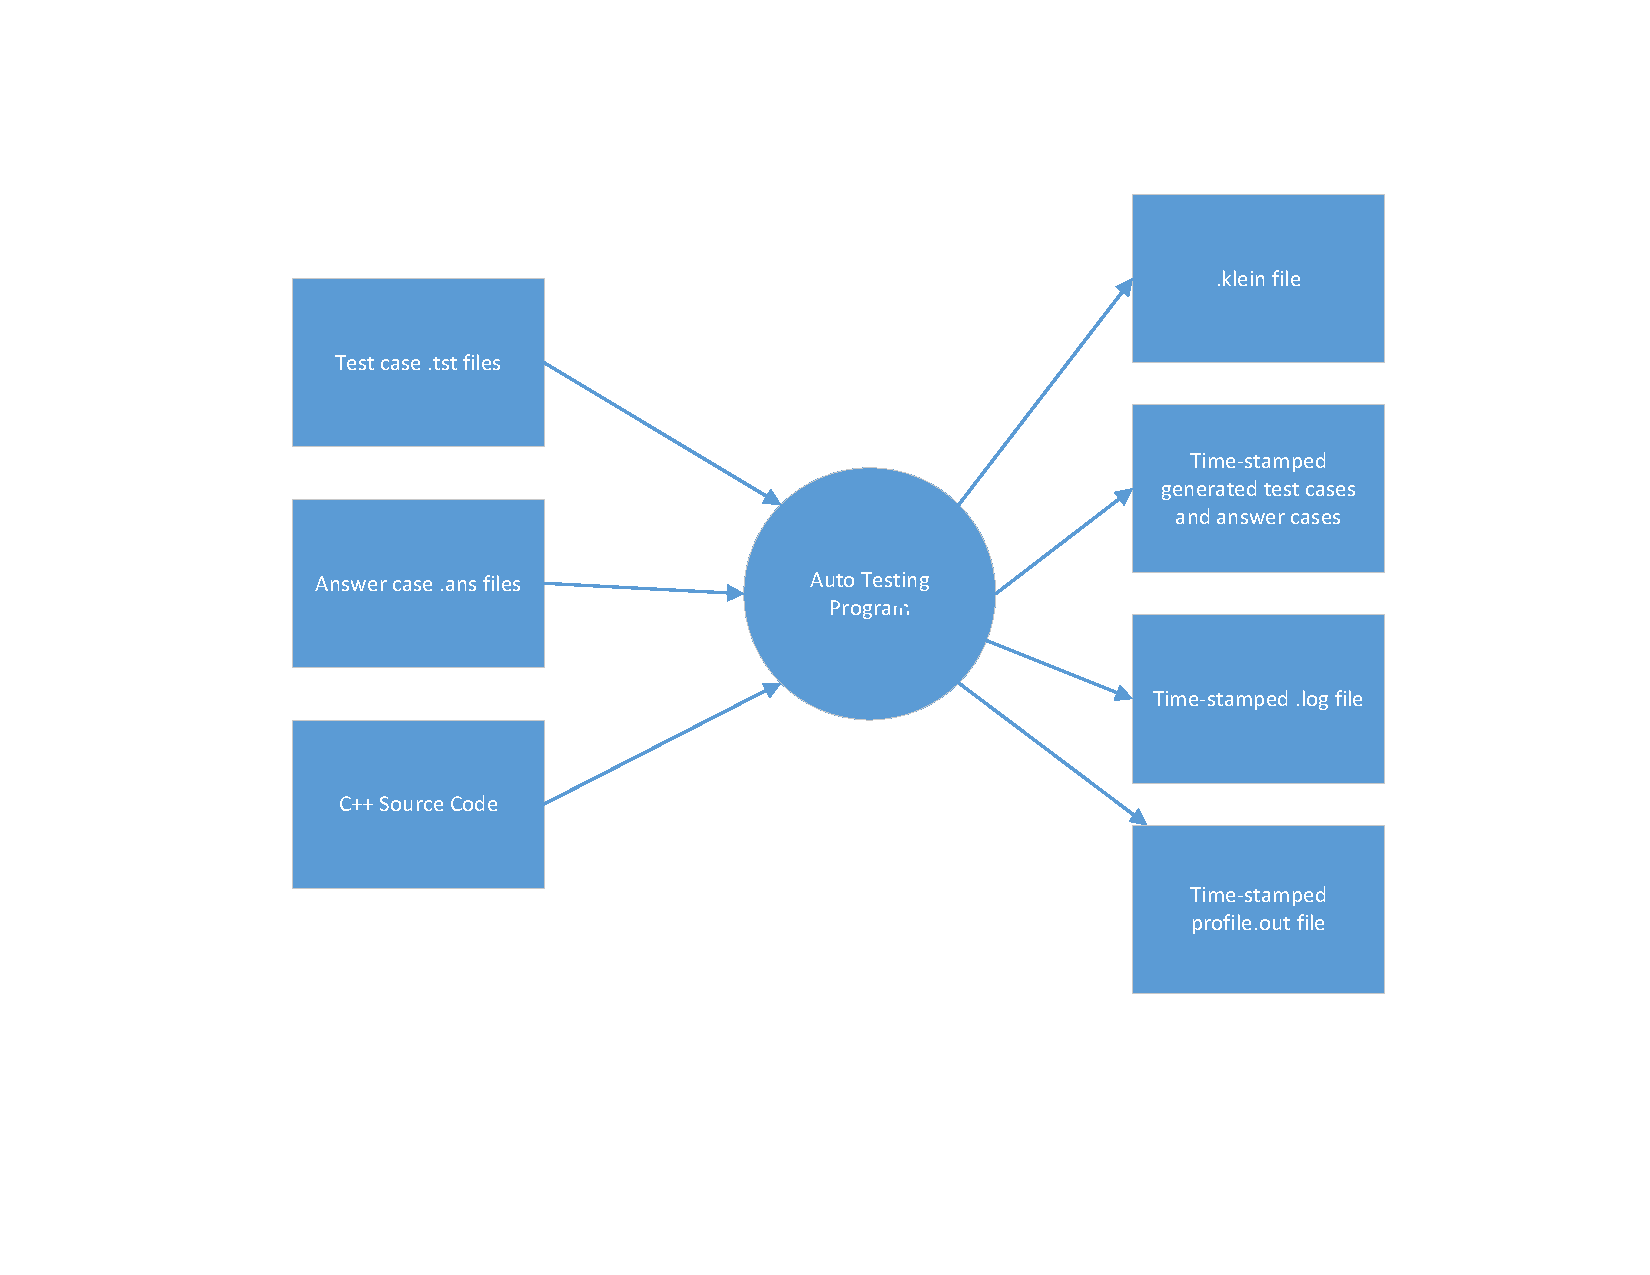
\includegraphics[width=1.0\textwidth]{./ArchitectDiagram}
\end{center}
\caption{Architecture Diagram for the Tester Application \label{arch_generic}}
\end{figure}


\subsection{Data Flow Diagram} 
%See Figure~\ref{dataflow}.



\begin{figure}[H]
\begin{center}
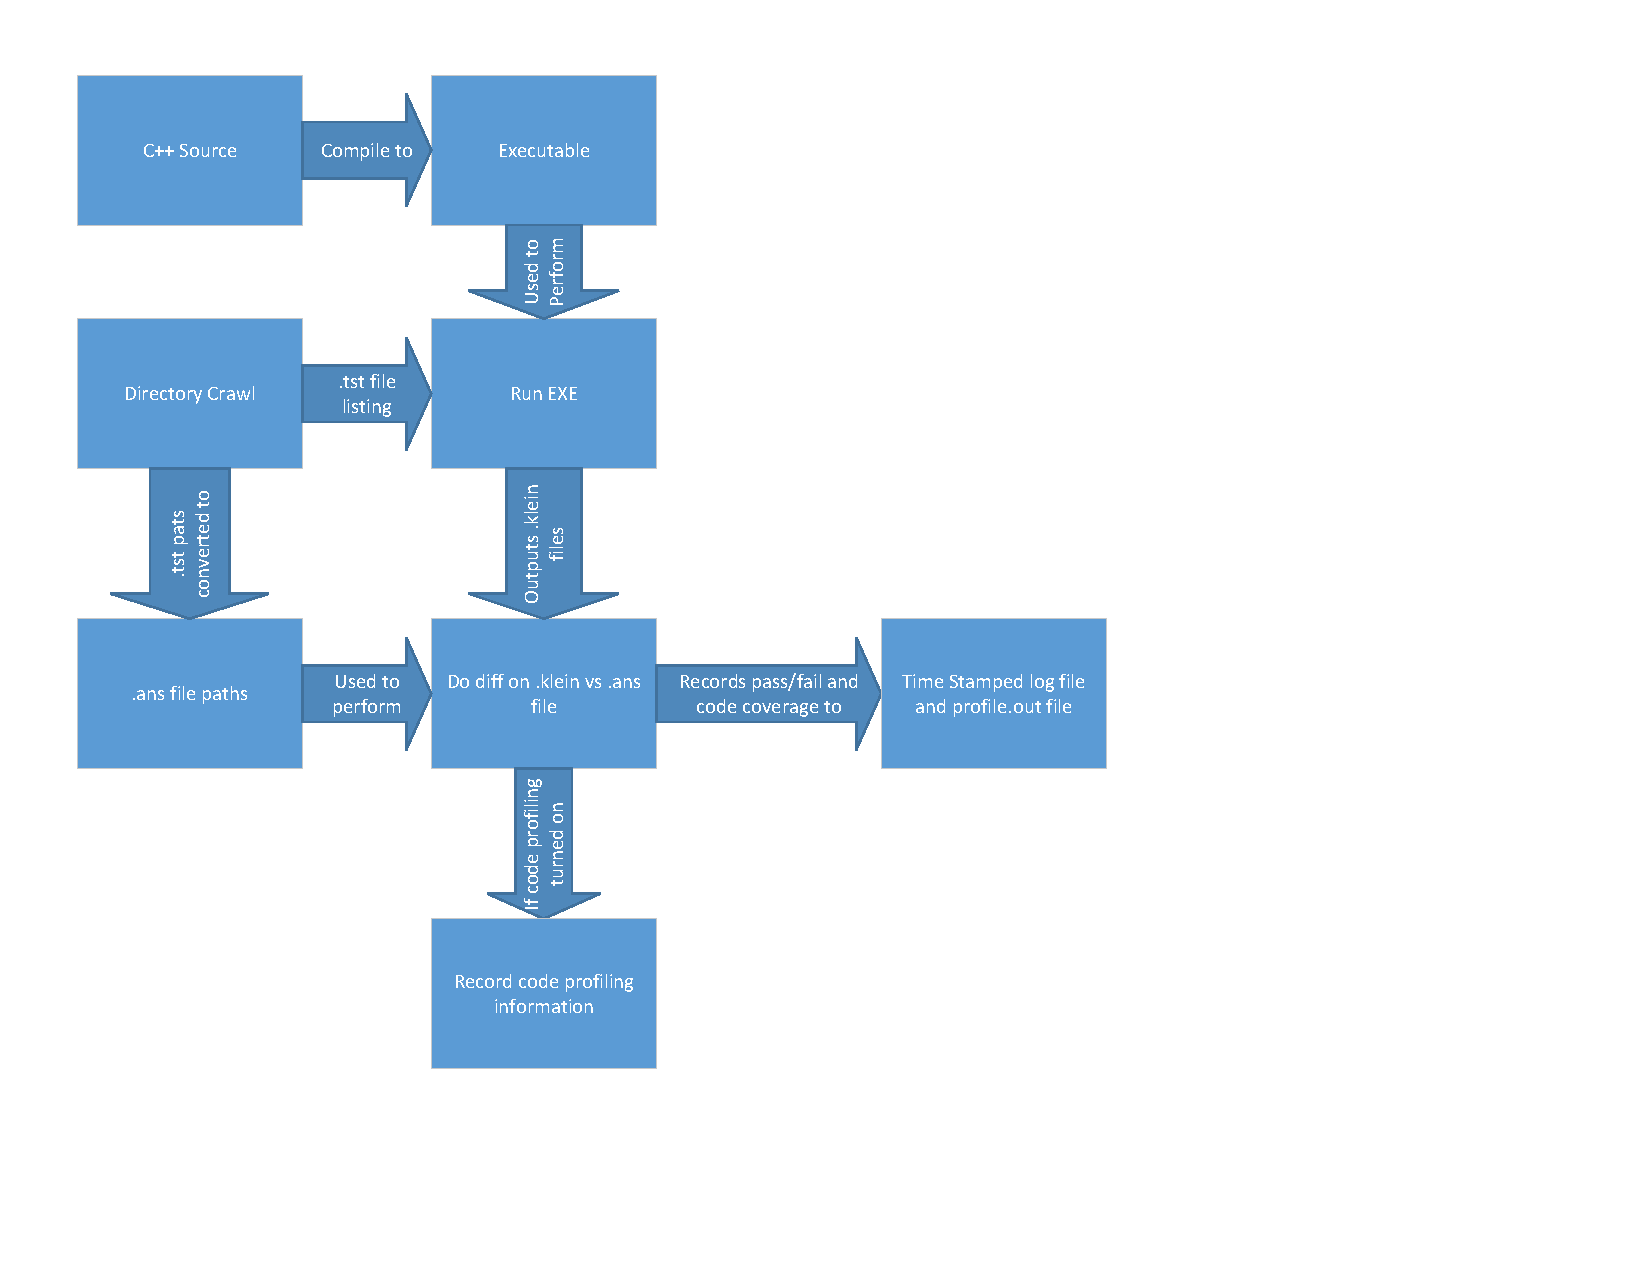
\includegraphics[width=0.75\textwidth]{./dataflow}
\end{center}
\caption{ Data Flow Diagram for the Tester Application \label{dataflow}}
\end{figure}


\subsection{Design Details}
The following function does the directory crawl and stores the relative path to 
 .tst file in the "dest" vector which is passed by reference. This is the recursive function that searches all sub-directories of the directory root which contains the executable program:
\begin{lstlisting}
// Recursive Directory Crawl
void TestSuite::dirCrawl(string targetExt, string dir, vector<string> &dest)
{
    // Open current directory.
    DIR * proc = opendir( dir.c_str() );

    if (NULL == proc)
    {
        return;
    }

    // Read current directory.
    dirent * entry = readdir(proc);

    do
    {
        // Make recursive calls to sub directories
        if(DT_DIR == entry->d_type)
        {
            string name = entry->d_name;
            if ( "." != name && ".." != name )
            {
                string newDir = dir + "/" + entry->d_name;
                dirCrawl( targetExt, newDir, dest );
            }
        }
        // Watch for files with .tst extension
        else if ( DT_REG == entry->d_type )
        {
            string fileName = entry->d_name;
            unsigned int extPos = fileName.rfind(".");
            if ( extPos != string::npos )
            {
                string ext = fileName.substr( extPos );
                if ( ".tst" == ext )
                {
                    fileName = dir + "/" + fileName;
                    cout << fileName << endl;
                    dest.push_back(fileName);
                }
            }
        }
    }while(entry=readdir(proc));

    closedir(proc);
}
\end{lstlisting}
Once this function has finished executing the destination vector contains a listing of all paths to .tst files to be run by the program being tested.



\section{Test Single Program Against Found Test Cases}

\subsection{Technologies  Used}
The only technology used in this section is C++ code.

\subsection{Component  Overview}
The purpose for this section is to compile the C++ code, loop through the list of .tst files in the directory, and check if the program output matches the .ans file output.

\subsection{Phase Overview}
Testing a program against located test cases is necessary in the second and third phases because we must be able to check the program's output against the .ans file to see if each test was a success or failure before program output can be prepared.

\subsection{ Architecture  Diagram}
Due to the small size of the application, a single diagram describing the architecture of the program is provided in Figure~\ref{arch_generic}

\subsection{Data Flow Diagram}
Due to the small size of the application, a single diagram describing the data flow for the program is provided in Figure~\ref{dataflow}.


\subsection{Design Details}
Testing the program may be broken down into three sections:
\begin{itemize}
	\item Compiling source C++ code
	\item Running C++ code against test case
	\item Determining if program output was correct for test case
\end{itemize}
The following function compiles the program using a system call to g++:
\begin{lstlisting}
//Function to compile c++ source code based on filename
bool TestSuite::compile_code( string filename )
{   string compile_instruction = "g++ "; // Form the string for the system call
    compile_instruction += filename;
    compile_instruction += " -o test_prog";

    system( compile_instruction.c_str() );

    return true;
}\end{lstlisting}
To run the executable against a test case another system call is made redirecting input from the test file and output to the ".klein" file:
\begin{lstlisting}
//Function to run c++ souce with redirected input/output
bool TestSuite::run_code( string test_file )
{   string run_instruction = "./test_prog < ";  //Form the string for the system call
    run_instruction += test_file;
    run_instruction += " > test_out.klein";

    system( run_instruction.c_str() );

    return true;
}
\end{lstlisting}
Finally, the program output file needs to be compared to the .ans file. This is also done with a system call to diff:
\begin{lstlisting}
//Function to do diff on answer file and test program output file
bool TestSuite::correct_answer( string ans_file )
{  string diff_instruction = "diff test_out.klein ";
    diff_instruction += ans_file;
 
   return (! system( diff_instruction.c_str() ) );
}
\end{lstlisting}
The only change to compare all the test files is to place the preceding functions in a loop and pass each new test file as a parameter to run\_code() which is done in run\_test() as follows:
\begin{lstlisting}
// Runs program with input from test files in testFiles vector.
void TestSuite::runTests()
{  numCorrect = numWrong = 0;
    pair<string, bool> result;

    vector<string>::iterator it;           // Iterate over test files.
    for ( it = testFiles.begin(); it != testFiles.end() ; it++ )
    {
        // Run program with given test file.
        run_code(*it);

        // Determine corresponding answer file.
        string ans = *it;
        ans.replace(ans.end()-4, ans.end(),answerExtension);

        // Populate results vector and counters.
        result.first = *it;
        if (correct_answer(ans))
        {
            result.second = true;
            numCorrect++;
        }
        else
        {
            result.second = false;
            numWrong++;
        }
        // Add results to vector.
        results.push_back(result);
    }
}
\end{lstlisting}
Upon completion, the TestSuite object contains counters for the number of correct and incorrect test cases to be used when outputting the log file.

\section{Record and Summarize Test Results }

\subsection{Technologies  Used}
The only technology used in this section is C++ code.

\subsection{Component  Overview}
After the test cases have been run a timestamped .log file needs to be produced. It should include if each test case passed or failed as well as the percentage of correct files along with the total number of correct and incorrect test cases.

\subsection{Phase Overview}
This component is included in the fourth phase of production. It was done last because the full output file could not be produced without knowing the results of all the test cases.

\subsection{ Architecture  Diagram}
Due to the small size of the application, a single diagram describing the architecture of the program is provided in Figure~\ref{arch_generic}


\subsection{Data Flow Diagram}
Due to the small size of the application, a single diagram describing the data flow for the program is provided in Figure~\ref{dataflow}.

\subsection{Design Details}
The formatted output is produced by the outputLogFile() function. It lists if each test case was a pass or failure along with overall test statistics. 



% !TEX root = SystemTemplate.tex

\chapter{System  and Unit Testing}

This section describes the approach taken with regard to system and unit testing. 

\section{Overview}
A file containing test case files and program files was provided by the client.  These
resources were used to test and troubleshoot the code during the development.

\section{Dependencies}
There are no external dependencies or frameworks for the program. Unit testing was carried out individually because the program was written without a predefined framework on which to test. 

\section{Test Setup and Execution}
The test cases and future test case format were provided by the client.  The latter is an important feature,
as one of the requirements of the application is that test cases must be able to be added and removed.

\begin{description}
\item [$\bullet$] Test case input is provided in the file test\_name.tst
\item [$\bullet$] Test case correct output is provided in the file test\_name.ans
\end{description}
% !TEX root = SystemTemplate.tex
\chapter{Development Environment}
The basic purpose for this section is to give a developer all of the necessary 
information to setup their development environment to run, test, and/or develop.

\section{Development IDE and Tools}
Development for this project was done in Qt Creator and other simple text editors such as VIM and Gedit. 
Two linux command line tools, gcov and gprof, were used in the project. They were used to create files the
user can analyze and determine a student's codes performance and what percent of the code was covered. 
The .pro file for the project is included with the source code.

In Sprint 2, the Qt Creator environment was dropped. In sprint 3 however, it was once again used by part 
of the group. 

\section{Source  Control}
The source control used in this project was Github for both Windows and Linux. A developer could connect 
to it by several ways; the first of which is to go to the Github website, where they were included as 
contributors to the repository where the code and documentation was stored. The second was to use either 
Linux or Windows to checkout the repository and use the push and pull functions off git to keep code and 
documentation updated.

\section{Dependencies}
Dependencies for this program include the c standard library and the POSIX API. The program also takes 
advantage of several Linux system calls. Therefore, it is assumed that it will be run in a Linux environment. 

\section{Build  Environment}
The program compiles with GCC into a single executable. This can either be done within Qt Creator or by using 
the Makefile provided with the source code. 

\section{Development Machine Setup}
This program is designed to run on a Linux based machine.
It was developed on machines running Fedora 20 and Fedora 19. On these developement machines we ensured the 
GCC compiler was up to date as to not cause any issues when compiling and running the program. 


% !TEX root = SystemTemplate.tex

\chapter{Release -- Setup -- Deployment}
This section contains subsections regarding specifics in releasing, 
setup, and/or deployment of the system. 


\section{Deployment Information and Dependencies}
Dependencies for this application include the c standard library and the POSIX API, both used for the
file system access in the test case finding portion of this program. This application also relies on Gcov and Gprof. Lastly, it relies on many Linux system calls.



\section{Setup Information}
A makefile will be provided with the application, which can be run using the command 'make' within the 
directory in which the makefile exists. To ensure a full rebuild of the system, run "make" with the "-B" argument.

The project is run by: \\
./tester [-g or -r] $\langle$ directory $\rangle$ [-p or empty]

The directory is the place where the test files, student programs, and golden source are stored. Student code is in subdirectories, and test files can be placed anywhere. Any test files generated by the program will be stored in the "tests" subdirectory.


\section{System  Versioning Information}
The system will be versioned with each Sprint of the class, incrementing the first decimal.

In addition to this, when a working version of the project was developed, that version was put into a branch with a time stamp. 
Additionally, every time a working bit of code was developed, it was put into the current branch with 
a description of what was currently working.

% !TEX root = SystemTemplate.tex

\chapter{User Documentation}

This section will contain the basis for any end user documentation for the system, 
and will cover the basic steps for the setup and use of the system.



\section{User Guide}
Usage of the Auto Tester is primarily concerned with the format and placement of the test case files. 
Test case files must be located in the same directory as the students program source, or in a subdirectory 
there of. The golden cpp, if present, must be given in the commandline, or be located in the first directory given. The .spec file must be present to enable menu driven testing.

\subsection{Test Case Files}
Files that contain the test cases themselves need to be given a .tst extension. The filename proceeding the 
extension will be used as the name of that test in the log file. The contents of the file will be the raw 
input to the student's program.

\subsection{Expected Output Files}
For each test case file, there needs to be a corresponding file that contains the expected output. This file 
must have the same name as the test case, but instead have a .ans extension.

\subsection{Auto Generated Tests}
The option to auto generate tests with a given 'golden cpp' will be available to the user. The user will run 
the Auto Tester with a given program, and then will go through a simple text based menu that will determine the 
parameters for the auto generated tests. The code will then place the .tst and .ans files in a subdirectory called "tests". The answer files will be generated by running the test files through the golden cpp. This product features menu driven testing, however, a .spec file must be present to enable this feature.

\subsection{Results}
The results for each student will be placed in a file with a .log extension, within the given student's directory. 
In addition, a complete log with the names of all the students and their pass/fail status and/or grade will be placed 
in the head directory. The filenames will be timestamped. Gcov information is put in each student log file. Gprof information, if enabled, will also be appended to the student log file.

\begin{figure}[H]
\begin{center}
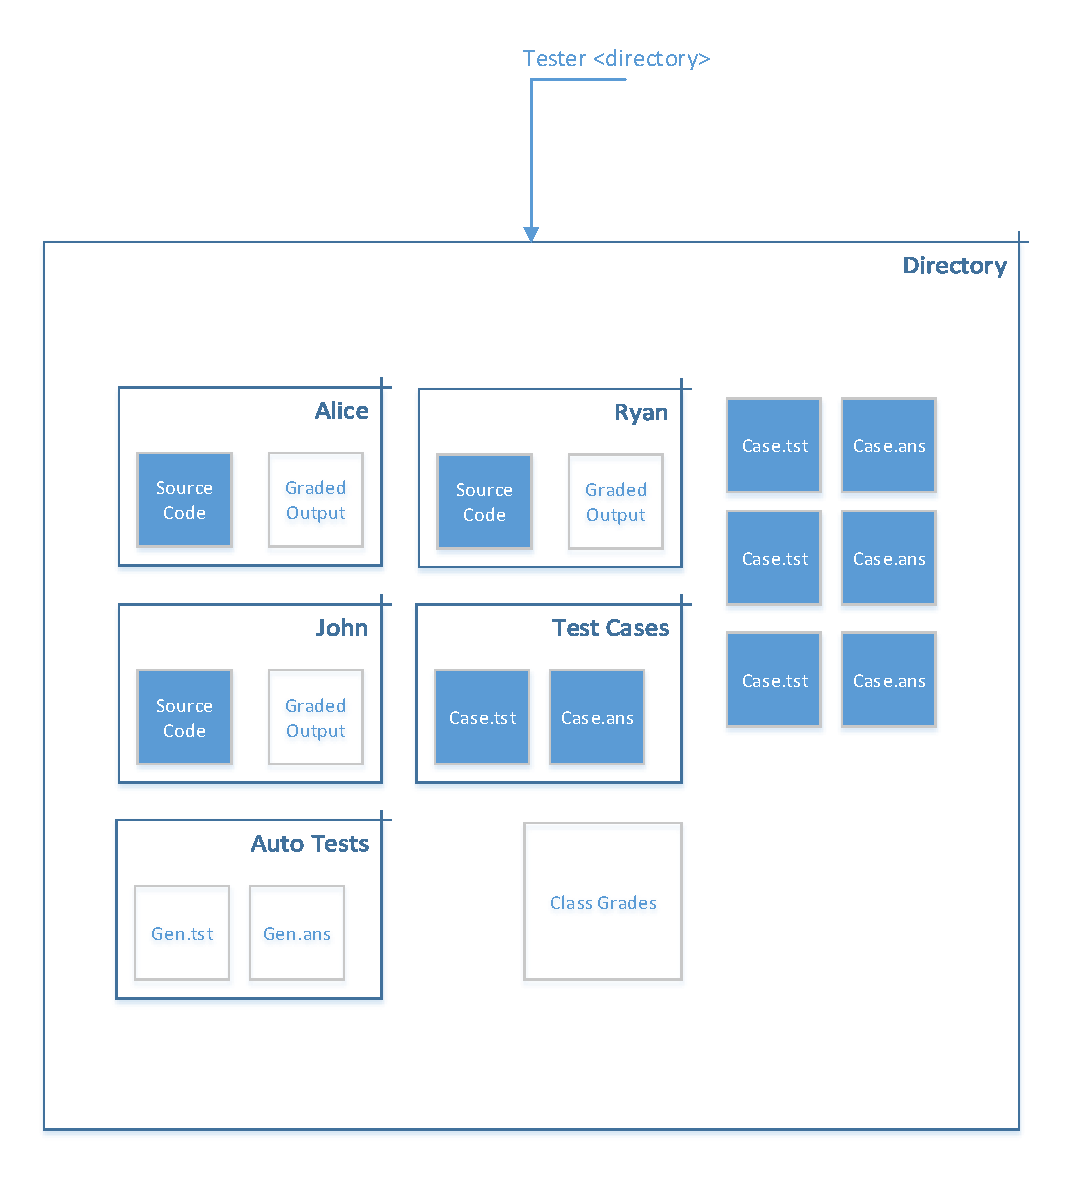
\includegraphics[width=0.75\textwidth]{./Dir_struct}
\end{center}
\caption{Example directory structure for runnning the tester \label{dir}}
\end{figure}

\section{Installation Guide}
To use the application, compile the source code using the supplied makefile.

After this is completed, the user should have an
executable file they can use by invoking the following: \\
./tester [-g or -r] $\langle$ directory $\rangle$ [-p or empty]

\section{Programmer Manual}
The code contained in the .cpp file is written in c++ and is to be compiled with g++.

% !TEX root = SystemTemplate.tex

\chapter{Class Index}
\section{Class List}
Here are the classes, structs, unions and interfaces with brief descriptions\-:\begin{DoxyCompactList}
\item\contentsline{section}{\hyperlink{class_poly}{Test\-Suite} \\*This class provides an interface for compiling and testing c++ programs against given test files }{\pageref{class_poly}}{}
\end{DoxyCompactList}
%\chapter{Class Documentation}
%\hypertarget{class_poly}{\section{Test\-Suite Class Reference}
\label{class_poly}\index{Test\-Suite@{Test\-Suite}}
}


This class provides an interface for compiling and testing c++ programs against given test files.  




{\ttfamily \#include $<$testsuite.\-h$>$}

\subsection*{Public Member Functions}
\begin{DoxyCompactItemize}
\item TestSuite ()
\item bool initTest (string program, string tstExt, string ansExt)\\
\textit{Initialize a testing session. Compiles the given program and locates all test and answer files.}  
\item void runTests()
	\textit{ Run the test.}
\item void outputLogFile() \\
	\textit{ Output a log file with results of test.}
\item bool menu\_tests(string spec\_file\_path) \\
 	\textit{generate menu driven test cases.}
\item void dirCrawl(string targetExt, string dir, vector\textless string\textgreater  \& dest)\\
 	\textit{get all files of target extension in a directory.}
 \item void helperfunc() \\
	 \textit{Run non menu drive test case generation.}
 \item void createSummary() \\
	 \textit{Record class test summary.}
 \item void presentatioMenu() \\
	 \textit{Run menu that gets options from user for either ignoring or not ignoring presentation errors.}
\end{DoxyCompactItemize}

\begin{DoxyCompactItemize}
\item 
testsuite.\-h\item 
testsuite.\-cpp\end{DoxyCompactItemize}




\backmatter
\chapter{Acknowledgement}
\label{SpecialThanks}  Thank you Dr. Logar for being awesome! 


\chapter{Supporting Materials}
This document will contain several appendices used as a way to separate out major 
component details, logic details, or tables of information.  Use of this structure 
will help keep the document clean, readable, and organized. 


%%% Since counters are different in the backmatter section
%%% we explicitly set the section number  (comment out to see effect)
\setcounter{section}{0}
% !TEX root = SystemTemplate.tex

\chapter{Sprint Reports}
\section{Sprint Report \#1}
As the development of this system was planned to be completed in one sprint, this is the final sprint review for the project. 
The review was conducted with the product owner, the technical lead, and the scrum master. \\

\subsection{Code Development}
The following were designed and written by Joseph Lillo:
\begin{description}
\item [TestSuite Class Declaration]- This class provides an interface for compiling and testing c++ programs against given test files.
\item [dirCrawl] - a function used to perform a recursive Directory Crawl \\ \\
\end{description}
The following were designed and written by Daniel Nix:
\begin{description}
\item [compile\_code] - a function used to compile c++ source code based on filename
\item [run\_code]- a function used to run c++ souce with redirected input/output
\item [correct\_answer]- a function used to do diff on answer file and test program output file \\  \\
\end{description}
The following were designed and written by Lisa Woody:
\begin{description}
\item [Software Documentation and formatting] - the final software write up for the project
\item [Log file output functions]-  functions later integrated into other functions upon team review of the program. \\
\end{description}
The following were designed and written by the Obfuscators as a team:
\begin{description}
\item [runTests] - a function used to run a program with input from test files in the testFiles vector
\item [reset]-  a function used to clear member data associated with testing session.
\end{description}




\subsection{Final Product Review}

The final application, having passed the final testing stages, was demonstrated.  \\
\begin{description}
\item [$\bullet$] Has every phase of the project been completed? 
\item Yes, each of the four phases of the project have been completed.
\item [$\bullet$]Have the phases been successfully integrated into the final product?
\item Yes, the phases are completely integrated into the final product.
\item [$\bullet$] Can the application run the client-provided test files without error?
\item Yes, the application compiles and no errors were found.
\item [$\bullet$] Does the final output match the intended and requested output?
\item Yes, the outputted log file matches the requested format.\\

\item Next, the documentation was reviewed. \\

\item [$\bullet$] Has the documentation been completely filled out and reviewed by each team member?
\item Yes, the documentation has been completed and reviewed. 
\item [$\bullet$] Does the product meet the requirements and needs of each user story?
\item Yes, the product fulfills the needs of each user story laid out in the documentation.
\item [$\bullet$] Does the product satisfy the product backlog and is it deemed deliverable by the product owner?
\item Yes, the product owner is deemed complete and deliverable by the product owner.\\

\item The team is happy with this sprint, and feels that next time it will be prepared for the newly learned Agile methodology and documentation style.\\
\end{description}

\section{Sprint Report \#2}
This sprint lasted from 2/21 to 3/22. The members of the Whitespace Cowboys recived the Obfuscator's first sprint code, 
analyzed it, and turned in a report to Dr. Logar conserning the workability and documentation of the given materials. 
One official scrum meeting was held to hold a planning poker and to assign coding tasks. These are were reflected using 
Trello cards. 

Several unofficial meetings were held, the last of which was used to go over what had not yet been 
completed and how the last steps would be taken to tie up the second sprint. During this last meeting, an unofficial 
code review was held concerning the completed functions, and github issues were worked out.

The code for the second sprint was officially completed on 3/23, with several last minute 
revisions made. Documentation was double checked, and the team made an effort to make sure 
the code was well documented and at least similar in coding standard.

\section{Sprint Report \#3}
N/A

% !TEX root = SystemTemplate.tex

\chapter{Industrial Experience}

\section{Resumes}

%    \includepdf[pages={1}]{report.pdf}  %% example of limited page include

%     \includepdf{resume1.pdf}
%     \includepdf{resume2.pdf}
%     \includepdf{resume3.pdf}

\section{Industrial Experience Reports}

\subsection{Name1}

% Report

\subsection{Name2}

% Report

\subsection{Name3}

% Report



\setcounter{section}{0}
%% !TEX root = SystemTemplate.tex

\chapter{Appendix}

Latex sample file:  

\section{Introduction}
This is a sample input file.  Comparing it with the output it
generates can show you how to produce a simple document of
your own.

\section{Ordinary Text}  % Produces section heading.  Lower-level
                                    % sections are begun with similar 
                                    % \subsection and \subsubsection commands.

The ends  of words and sentences are marked 
  by   spaces. It  doesn't matter how many 
spaces    you type; one is as good as 100.  The
end of   a line counts as a space.

One   or more   blank lines denote the  end 
of  a paragraph.  

Since any number of consecutive spaces are treated like a single
one, the formatting of the input file makes no difference to
      \TeX,         % The \TeX command generates the TeX logo.
but it makes a difference to you.  
When you use
      \LaTeX,       % The \LaTeX command generates the LaTeX logo.
making your input file as easy to read as possible
will be a great help as you write your document and when you
change it.  This sample file shows how you can add comments to
your own input file.

Because printing is different from typewriting, there are a 
number of things that you have to do differently when preparing 
an input file than if you were just typing the document directly.  
Quotation marks like 
       ``this'' 
have to be handled specially, as do quotes within quotes: 
       ``\,`this'                  % \, separates the double and single quote.
        is what I just 
        wrote, not  `that'\,''.  

Dashes come in three sizes: an 
       intra-word 
dash, a medium dash for number ranges like 
       1--2, 
and a punctuation 
       dash---like 
this.

A sentence-ending space should be larger than the space between words
within a sentence.  You sometimes have to type special commands in
conjunction with punctuation characters to get this right, as in the
following sentence.
       Gnats, gnus, etc.\    % `\ ' makes an inter-word space.
       all begin with G\@.   % \@ marks end-of-sentence punctuation.
You should check the spaces after periods when reading your output to
make sure you haven't forgotten any special cases.
Generating an ellipsis 
       \ldots\    % `\ ' needed because TeX ignores spaces after 
                  % command names like \ldots made from \ + letters.
                  %
                  % Note how a `%' character causes TeX to ignore the 
                  % end of the input line, so these blank lines do not
                  % start a new paragraph.
with the right spacing around the periods 
requires a special  command.  

\TeX\ interprets some common characters as commands, so you must type
special commands to generate them.  These characters include the
following: 
       \$ \& \% \# \{ and \}.

In printing, text is emphasized by using an
       {\em italic\/}  % The \/ command produces the tiny extra space that
                       % should be added between a slanted and a following
                       % unslanted letter.
type style.  

\begin{em}
   A long segment of text can also be emphasized in this way.  Text within
   such a segment given additional emphasis 
          with\/ {\em Roman} 
   type.  Italic type loses its ability to emphasize and become simply
   distracting when used excessively.  
\end{em}

It is sometimes necessary to prevent \TeX\ from breaking a line where
it might otherwise do so.  This may be at a space, as between the
``Mr.'' and ``Jones'' in
       ``Mr.~Jones'',        % ~ produces an unbreakable interword space.
or within a word---especially when the word is a symbol like
       \mbox{\em itemnum\/} 
that makes little sense when hyphenated across 
       lines.

Footnotes\footnote{This is an example of a footnote.}
pose no problem.

\TeX\ is good at typesetting mathematical formulas like
       \( x-3y = 7 \) 
or
       \( a_{1} > x^{2n} / y^{2n} > x' \).
Remember that a letter like
       $x$        % $ ... $  and  \( ... \)  are equivalent
is a formula when it denotes a mathematical symbol, and should
be treated as one.

\section{Displayed Text}

Text is displayed by indenting it from the left margin.
Quotations are commonly displayed.  There are short quotations
\begin{quote}
   This is a short a quotation.  It consists of a 
   single paragraph of text.  There is no paragraph
   indentation.
\end{quote}
and longer ones.
\begin{quotation}
   This is a longer quotation.  It consists of two paragraphs
   of text.  The beginning of each paragraph is indicated
   by an extra indentation.

   This is the second paragarph of the quotation.  It is just
   as dull as the first paragraph.
\end{quotation}
Another frequently-displayed structure is a list.
The following is an example of an {\em itemized} list.
\begin{itemize}
   \item  This is the first item of an itemized list.  Each item 
          in the list is marked with a ``tick''.  The document
          style determines what kind of tick mark is used.

   \item  This is the second item of the list.  It contains another
          list nested inside it.  The inner list is an {\em enumerated}
          list.
          \begin{enumerate}
              \item This is the first item of an enumerated list that
                    is nested within the itemized list.

              \item This is the second item of the inner list.  \LaTeX\
                    allows you to nest lists deeper than you really should.
          \end{enumerate}
          This is the rest of the second item of the outer list.  It
          is no more interesting than any other part of the item.
   \item  This is the third item of the list.
\end{itemize}
You can even display poetry.
\begin{verse}
   There is an environment for verse \\    % The \\ command separates lines
   Whose features some poets will curse.   % within a stanza.

                           % One or more blank lines separate stanzas.

   For instead of making\\
   Them do {\em all\/} line breaking, \\
   It allows them to put too many words on a line when they'd 
   rather be forced to be terse.
\end{verse}

Mathematical formulas may also be displayed.  A displayed formula is
one-line long; multiline formulas require special formatting
instructions.
   \[  x' + y^{2} = z_{i}^{2}\]
Don't start a paragraph with a displayed equation, nor make
one a paragraph by itself.

\section{Build process}

To build \LaTeX\ documents you need the latex program.  It is free and available on all operating systems.   Download and install.  Many of us use the TexLive distribution and are very happy with it.    You can use a editor and command line or use an IDE.  To build this document via command line:

\begin{verbatim}
alta>  pdflatex SystemTemplate
\end{verbatim}
If you change the bib entries, then you need to update the bib files:
\begin{verbatim}
alta>  pdflatex SystemTemplate
alta>  bibtex SystemTemplate
alta>  pdflatex SystemTemplate
alta>  pdflatex SystemTemplate
\end{verbatim}


\section*{Acknowledgement}
Thanks to Leslie Lamport





%\bibliography{designrefs.bib}
%\bibliographystyle{plain}



\end{document}
